\documentclass[letterpaper,12pt]{article}
\usepackage[utf8]{inputenc}
\usepackage{fullpage}
\usepackage{courier}
\usepackage[margin=0.75in]{geometry}
\usepackage{listings}
\usepackage{color}
\usepackage{graphicx}
\usepackage[width=5in]{caption}
\usepackage{hyphenat}
\usepackage[section]{placeins}

% Format a sectionless paragraph
\newcommand*\unparagraph{
	\par
	\nopagebreak
	\vskip3.25ex plus1ex minus.2ex
	\noindent
}

% define extra colors
\definecolor{dkgreen}{rgb}{0,0.6,0}
\definecolor{purple}{RGB}{159,0,197}

% define the code listing format
\lstset{
	language=C++,
	basicstyle=\footnotesize\ttfamily,
	backgroundcolor=\color{white},
	showspaces=false,
	showstringspaces=false,
	frame=none,
	tabsize=3,
	keywordstyle=\color{purple},
	commentstyle=\color{dkgreen},
	stringstyle=\color{blue},
	escapeinside={\%*}{*)}
}

% define the title/header
\title{\Large CS 1428 Honors\\Style Guide} 
\author{Jared Wallace}
\date{}

\begin{document}

\maketitle

\vspace{30mm}

\section*{Indentation}
Make sure you use spaces, not tabs. Tabs are evil.
I recommend you use four spaces as your indentation level, but as long
as you are consistent, I don't really care.

\section*{Naming}
Variables should be all lowercase, with the underscore as a separator
\begin{lstlisting}
    float interest_rate = 0.0;
\end{lstlisting}
Please make your variable names
descriptive
\begin{lstlisting}
    // this
    float price_of_meal = 8.25;
    // not this
    float prcml = 8.25;
\end{lstlisting}
Constants should be all uppercase
\begin{lstlisting}
    const float TAX_RATE = 7.75;
\end{lstlisting}
Functions should be camel case, starting with a capital
\begin{lstlisting}
    void MyAwesomeFunction( int price, float tax)
    {
        // awesome stuff here
    }
\end{lstlisting}
\section*{Comments}
Learning how to comment well is more art than science. You don't want overly
verbose comments cluttering your code, but you still want to provide assistance to
those who are trying to understand it. These are some guidelines.
\begin{itemize}
    \item Explain tricky bits of code, like complex calculations
    \item For functions, explain what conditions are needed for the function
        to work correctly (like the incoming data must be a certain type, or a 
        certain global constant must exist, etc) as well as what the function does
        and what conditions will be true upon exit from the function. For example:
        \begin{lstlisting}
            /*  This function calculates the grand total and tip for a meal
             *  Precondition: the price argument should be a non-negative float,
             *      the tip_amount argument should be an integer percentage (like 10), and the
             *      TAX_RATE constant must have been declared.
             *  Postcondition: the function will return the appropriate tip amount.
             */
            float CalculateTip( int tip, float price)
            {
                // awesome stuff here
            }
        \end{lstlisting}

    \item Try to anticipate difficult to understand sections of code, and explain them
\end{itemize}

\section*{General requirements}
\begin{itemize}
    \item Do not exceed 80 characters on any given line. Word wrap is ugly
    \item Always include your standard header at the top of your file
        \begin{lstlisting}
            /*
             *  Name: Jared Wallace
             *  Date: 08-26-2014
             *  Lab:  1
             *  Description: This program will solve world hunger, end war,
             *      and make everyone rich.
             */
        \end{lstlisting}
    \item Separate logical sections of code with a single blank line.
    \item Put two blank lines between functions.
    \item Always initialize variables when instantiated. Same for arrays.
\end{itemize}
% Comic at the bottom
\begin{figure}[ht!]
	\centering
	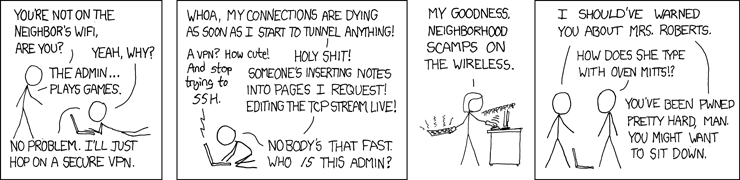
\includegraphics[width=5in]{1337_part_1.png}
    \caption*{If you're not cool enough to do it manually, you can look up tools like Upside-Down-Ternet for playing games with people on your wifi.}
\end{figure}
\end{document}
